\chapter{Projekt systemu i elementy implementacji}
W~tym rozdziale zaprojektuję oprogramowanie realizujące cele opisane w~punkcie~\ref{lib-requirements}.
Zaproponuję sposób realizacji, możliwości i~ograniczenia poszczególnych jego elementów. Dla części komponentów stworzę prototypy.

\section{Specyfikacja wymagań systemowych (SWS)}
Z~celów tej pracy zawartych w~punkcie~\ref{lib-requirements} stworzyłem standardową listę konkretnych wymagań dla zespołu inżynierów, czyli mnie samego.
Organizując niniejszą sekcję wzorowałem się na specyfikacji wymagań systemowych opisanej w~prezentacji ,,Inżynieria Wymagań'' Jarosława Kuchty, z~przedmiotu ,,Dokumentacja i~Jakość Oprogramowania''\cite{kuchta}.


\subsection{Wstęp i~opis informacyjny}
Jako rozbudowana sekcja wstępu SWS oraz ,,szczegółowy opis problemów do rozwiązania'' służyły poprzednie rozdziały niniejszej pracy.


\subsubsection{Diagram przepływu najwyższego poziomu}
Diagram~\ref{fig:project-overview} przedstawia ogólne działanie systemu w~trakcie wywoływania zdalnej metody. Jest to główna funkcja mojego projektu. Funkcja drugorzędna -- tłumaczenie danych, również została ujęta.


Widoczny na schemacie klient jest jednym z~wielu, które mogą być stworzone przez kod korzystający z~mojej biblioteki.
Obiekt każdego klienta spełnia jakiś zadany interfejs. Robi to przez opakowywanie parametrów, zaadresowanie ich, wysłanie do obiektu faktycznie wykonującego kod i~odebranie wyniku.
Interfejs klienta i obiektu zdalnego są zgodne, chodź napisane w~różnych językach na różne platformy. Aby zminimalizować nakład pracy programisty, najlepiej byłoby, gdyby interfejs po stronie klienta (.NET) był generowany z~wersji serwerowej (Java, Android).
Tak samo jak w~przypadku interfejsów wygląda sprawa klas przekazywanych do metod jako parametry -- także muszą być zgodne, najlepiej automatycznie tłumaczone.
Typy przetłumaczone na schemacie oznaczone są apostrofem.
Kod kliencki nie musi zawierać tłumaczenia implementacji zdalnych interfejsów.
Współdzielone definicje klas danych i~interfejsów są niezbędne, aby uzyskać polimorfizm metod zdalnych.

Serwer jest tworzony przez kod kliencki i~nasłuchuje na żądania na zadanym interfejsie sieciowym. Może to być dowolna technologia pozwalająca na dwustronne wysyłanie wiadomości, np.\ TCP, HTTP, SSL/TLS, czy też strumienie w~pamięci (rozwiązanie lokalne).
Na schemacie serwer posiada tylko jeden obiekt zdalny klasy \texttt{Implementacja A}, ale faktycznie może posiadać ich wiele.

\begin{figure}
	\centering
		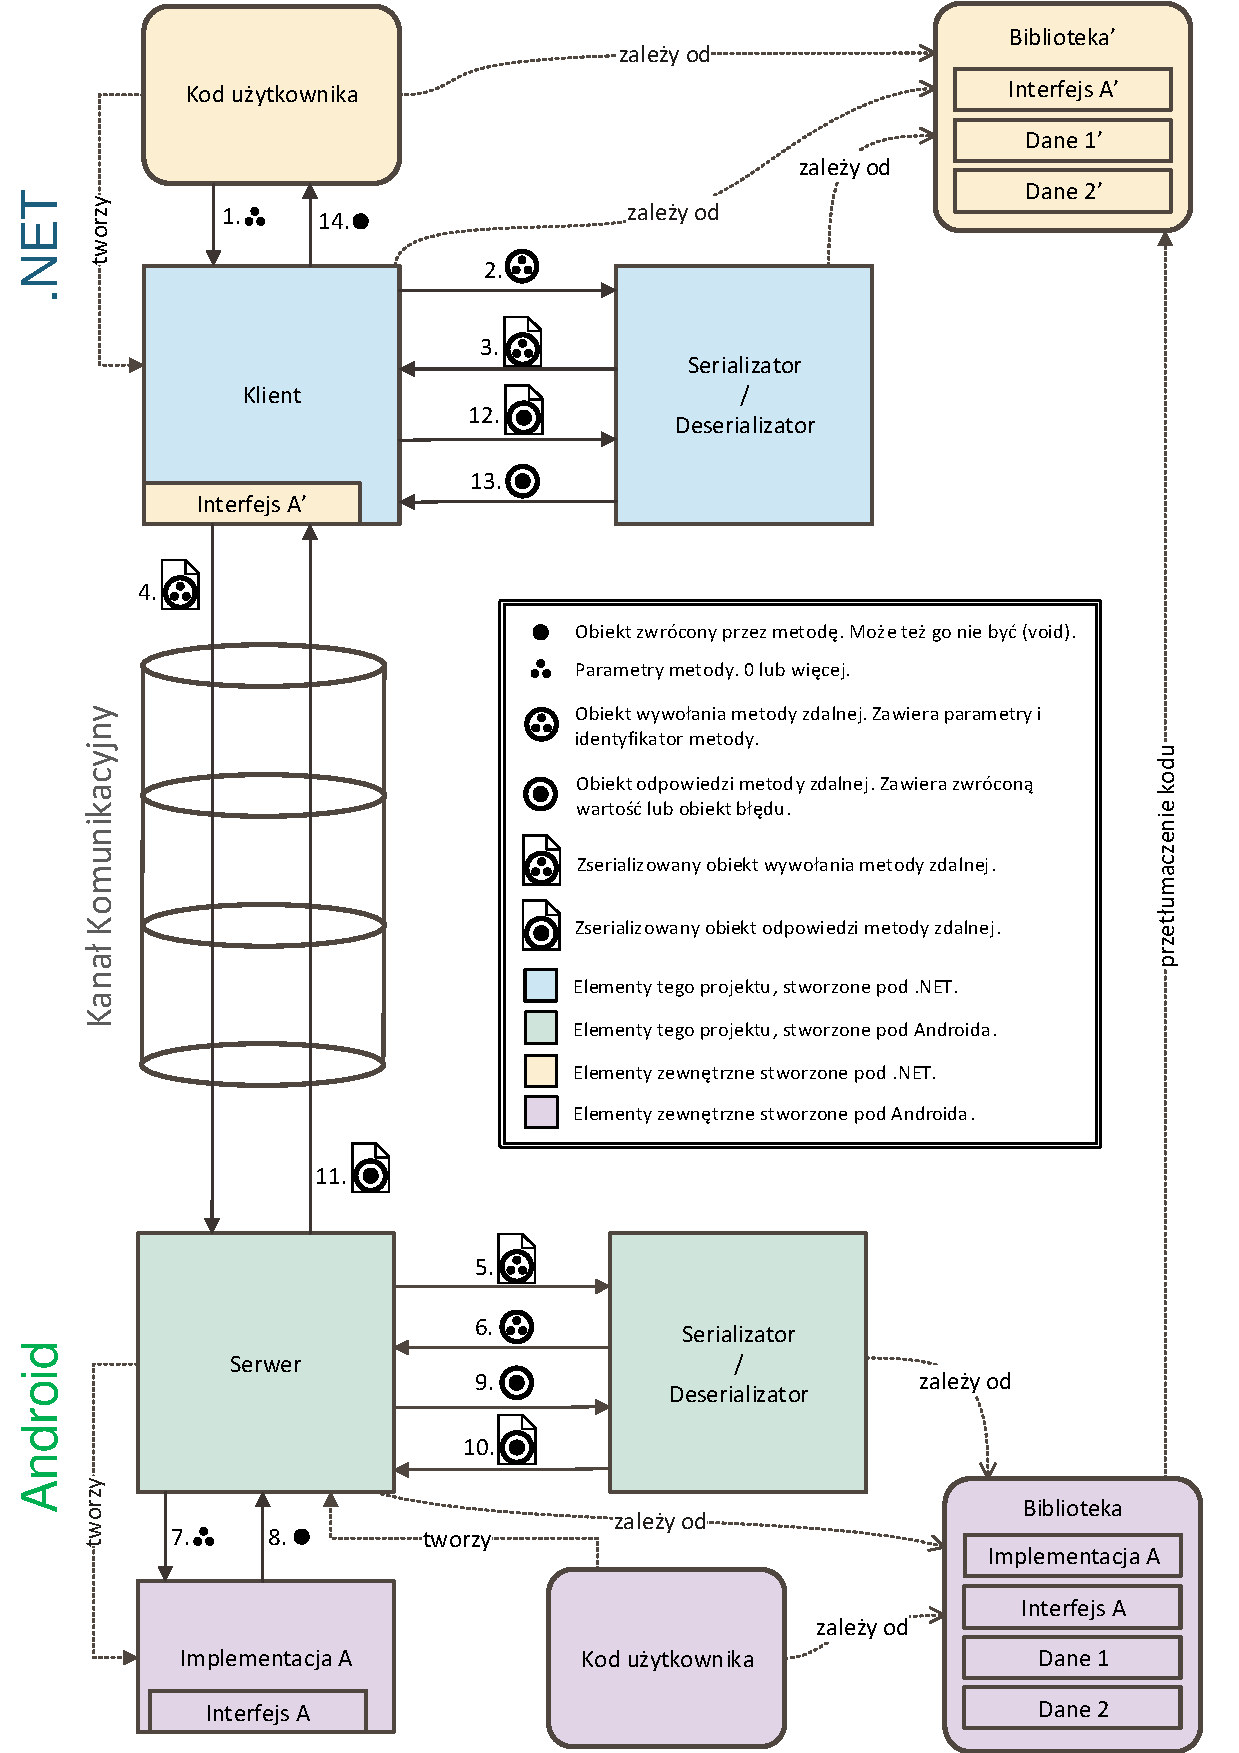
\includegraphics[scale=0.8]{img/schematy/schemat-dzialania-magisterki.pdf}
	\caption{Ogólny schemat projektu.}
	\label{fig:project-overview}
\end{figure}


\subsubsection{Reprezentacja zawartości informacyjnej}
Nie można właściwie mówić o~zawartości informacyjnej systemu, ponieważ takiej nie będzie.
Przez mój system dane będą jedynie przepływać.


\subsubsection{Opis interfejsów systemowych}
\begin{itemize}
	\item Jako, że to, co tworzę będzie kolekcją bibliotek Javy i~C\# będą one mogły być ładowane, a~ich klasy wykorzystywane przez zewnętrzne aplikacje.
	\item Niezależne narzędzie do generacji kodu będzie opatrzone w~interfejs linii poleceń.
\end{itemize}


\subsection{Wymagania funkcjonalne}
% WYMAGANIA POMIJANE:
% reliable sessions (w sumie też by mi się przydał jakiś mechanizm, który umożliwi komunikację w niestabilnym środowisku Internetu)
% \url{http://blogs.msdn.com/b/shycohen/archive/2006/02/20/535717.aspx} \\

\subsubsection{Ogólne}

\begin{description}
\itemtitle{Serializacja danych z zachowaniem informacji o typach}
Zserializowane reprezentacje obiektów muszą zawierać informacje o~typach wtedy, kiedy nie wynika ona jednoznacznie z~kontekstu.
Np.\ przy zwracaniu ze zdalnej metody obiektu klasy dziedziczącej po tym, zdeklarowanym w~interfejsie tejże metody.
To wymaganie dotyczy zarówno strony klienta jak i~serwera.
Deserializacja powinna być komplementarna i~ze stworzonych reprezentacji odtwarzać obiekty o~odpowiednich typach i~z~poprawnymi danymi.
Taka metoda serializacji i~deserializacji jest warunkiem działania polimorficznych metod.

\itemtitle{Tłumaczenie kodu}
Zrealizowane jako niezależne narzędzie.
Tłumaczenie kodu zmniejszyłoby nakład pracy programisty, który bez tego musiałby sam stworzyć odpowiadające klasy danych w~obu językach.
Klasy i~pola nie znajdujące odpowiednika są pomijane w~trakcie tłumaczenia.
Tłumaczenie powinno się odbywać z~Javy do C\#, ponieważ w~Javie będzie więcej kodu (kod implementacji zdalnych metod).
%Jeśli w danej klasie są inne klasy z zewnętrznej biblioteki, to trzeba też przetłumaczyć te. Trzeba dostarczyć kod wszystkich.
%Jeśli jedno ogniwo jest nieprzetłumaczalne to można pominąć pole z ostrzeżeniem.
\end{description}

\subsubsection{Serwer}

\begin{description}

\itemtitle{Komunikacja z~klientem}
Serwer powinien nasłuchiwać na żądania od klientów na zadanym dwustronnym kanale komunikacyjnym.
Konkretny typ kanału (TCP, SSL, HTTP, itp.) nie jest ważny.
Może przyjmować wywołania metod i~przekierowywać je do obiektów zdalnych (względem klienta).
Przekazuje do klientów zwracane wartości.

\itemtitle{Wystawianie metod publicznych zadanych obiektów ,,na zewnątrz''}
Kod serwera ma przyjmować dowolny obiekt i~umożliwiać zdalnym klientom wywoływanie jego publicznych metod.
Parametry tych metod muszą być przetłumaczalne na kod klienta.

% Można się też zastanowić nad singletonami.
\itemtitle{Tworzenie zdalnych obiektów na życzenie klienta}
Po otrzymaniu specjalnego żądania kod serwera powinien stworzyć obiekt implementujący zadany interfejs i~zwrócić jego identyfikator. Klient będzie mógł wywoływać zdalnie metody na stworzonym obiekcie.

\itemtitle{Niszczenie zdalnych obiektów na życzenie klienta}
Specjalne żądanie zawierające identyfikator obiektu powinno powodować jego zwolnienie i~uniemożliwienie z~nim dalszej komunikacji.

\itemtitle{Polimorfizm parametrów metod zdalnych}
Metody zdalne muszą obsługiwać parametry wszystkich typów zgodnych ze spodziewanym. Dla przykładu, metoda przyjmuje parametr typu A, więc powinna przyjąć też parametry wszystkich typów dziedziczących po A.

\itemtitle{Przeciążanie metod zdalnych}
Metody zdalne mogą być przeciążane, tj.\ dwie metody mogą mieć tę samą nazwę, ale inny zestaw parametrów.

\itemtitle{Komunikacja z systemem Android}
Obiekty zdalne muszą mieć możliwość wywoływania metod z~API Androida.

\end{description}

\subsubsection{Klient}

\begin{description}

\itemtitle{Tworzenie obiektów klienckich}
Biblioteka po stronie .NET musi być w~stanie dynamicznie stworzyć obiekt klienta dla obiektu zdalnego.
Każdy klient spełnia jakiś zadany interfejs.

\itemtitle{Nawiązywanie sesji z~serwerem}
Obiekt klienta nawiązuje kontakt z~serwerem poprzez dowolny dwustronny kanał komunikacyjny (na którym serwer nasłuchuje).
Następnie żąda od serwera stworzenia dla siebie zdalnego obiektu.
Wszystkie metody z~interfejsu zdalnego wywoływane na kliencie są przekazywane do jednego obiektu zdalnego.
Zwolnienie obiektu klienta powoduje zwolnienie obiektu zdalnego.

\itemtitle{Konsumowanie polimorficznych metod zdalnych}
Klient wykonuje metody implementowanego przez siebie interfejsu przez delegację (i~wysłanie) ich do obiektu zdalnego.
Wysłanie poprzedzane jest serializacją, podczas której muszą zostać zachowane informacje o~typach parametrów oraz ich ewentualnych obiektach składowych.

\end{description}


\subsection{Wymagania niefunkcjonalne}

\begin{description}

\itemtitle{Serwer na Androidzie}
Kod serwera musi działać na platformie Android.

\itemtitle{Klient w~.NET pod Windows}
Kod klienta musi działać na platformie .NET\@.

\itemtitle{Wydajność serwera}
Nie musi być duża, jako, że nie jest priorytetem projektu. Wystarczy jednoczesna obsługa pięciu (5) klientów.

\itemtitle{Rozszerzalność metod zdalnych bez ingerencji w oryginalny kod}
Funkcjonalność metod zdalnych powinna być rozszerzalna bez ingerencji w~ich kod dzięki mechanizmom programowania obiektowego.
Przykładem jest możliwość przyjmowania przez metodę zdalną obiektu klasy dziedziczącej po spodziewanym typie parametru, bez potrzeby jakiejkolwiek ingerencji w~kod metody, aby mogła rozumieć nową klasę.
Jednak definicja nowej klasy musi być dostępna zarówno dla klienta, jak i~serwera.

\itemtitle{Łatwość użytkowania}
Budowanie i~korzystanie z~bibliotek, które powstaną w~trakcie realizacji tego projektu, powinno być proste i~intuicyjne.

\end{description}



\section{Używana konfiguracja sprzętowa i~narzędzia (TODO)}
Przed przystąpieniem do omawiania komponentów rozwiązania warto wspomnieć o~tym, na jakiej konfiguracji sprzętowej będę wytwarzał prototypy. Przedstawię też narzędzia, z których korzystałem.
Prototypy wykonywałem na 64-bitowym Windowsie 7 i emulatorze Androida takim a takim.

\subsection{IDE}
Eclipse z ADT
Visual Studio 2013


\subsection{Emulator Androida}
\label{android-emulator}
Używałem Eclipsa z wtyczką do Androida z~\url{http://developer.android.com/sdk/index.html}.
Ściągnąłem i używam narzędzia dla Androida 4.4.2.

Emulator chodził na obrazie do tych narzędzi, czyli \emph{ARM EABI v7a}. Emulator standardowy od Google.\footnote{Jest jeszcze alternatywny emulator wzmiankowany na stronach Xamarina -- Genymotion, \url{http://www.genymotion.com/}. Kto wie, może są jeszcze inne. Można też chyba w~VirtualBoxie hostować Androida na x86}
Używam ARMowego, bo więcej telefonów jest właśnie na nim. Zdażają się też drobne rozbieżności działania niektórych niskopoziomowych aplikacji względem obrazu na architekturę x86 (\emph{Intel x86 Atom}).
Konfiguracja używanej AVD: (w obrazku)
Forward portu


%Co to? Jakie wymagania spełnia? Co by wchodziło w tego skład lub ogólny sposob realizacji? Realizacja prototypu. Ograniczenia?
\section{Wspólny format informacji o typach (TODO)}
Zarówno część na Androidzie jak i~.NET musi tak samo oznaczać typy obiektów w~zserializowanych obiektach.
Jest to podstawa do uzyskania polimorficznych zdalnych metod.
Wymaga zgodnych serializatorów po obu stronach kanału komunikacyjnego.


\subsection{Spełniane wymagania}
Takie i takie i takie


\subsection{Realizacja}
Chcę to zrobić przez dobranie serializatorów po obu stronach i~odpowiednią ich konfigurację. Ewentualnie będę ingerował w~ich kod.
Myślę o~Jackson po stronie Androida i~DataContractJsonSerializer lub JSON.NET po stronie .NET\@.

Alternatywnym sposobem byłby parser--nakładka. Przetwarzał by on gotowy dokument JSON przygotowany przez JSON.NET na format Jacksona i na odwrót. Byłoby to wolne, ale wymagałoby może mniej ingerencji w~kod. A~pozwalałoby na uzyskanie pełnej zgodności.

\subsubsection{Porównanie sposobów serializacji w JSON.NET i Jackson}
Jackson serializuje tak a JSON.NET tak (wypunktować):
BLABLABLABLA
Żeby były zgodne trzeba zrobić to i to (wypunktować)

TABLICA
\begin{lstlisting}[float, frame=single, caption={Jackson daje.}, label=kod:jackson-serilization]
[
  "[Ljava.lang.Object;",
  [
    28,
    "jakis tekst",
    {
      "@class":"uniserialjava.DaneA",
      "numberA":13,
      "stringA":"domyslny"
    },
    {
      "@class":"uniserialjava.DaneB",
      "numberA":13,
      "stringA":"domyslny",
      "numberB":5.25
    }
  ]
]
\end{lstlisting}

\begin{lstlisting}[float, frame=single, caption={JSON.NET daje.}, label=kod:json-net-serilization]
{
  "$type": "System.Object[], mscorlib",
  "$values": [
    28,
    "jakis tekst",
    {
      "$type": "UniSerialDotNet.DaneA, UniSerialDotNet",
      "liczbaA": 13,
      "tekstA": "domyslny"
    },
    {
      "$type": "UniSerialDotNet.DaneB, UniSerialDotNet",
      "liczbaB": 5.25,
      "liczbaA": 13,
      "tekstA": "domyslny"
    }
  ]
}
\end{lstlisting}


LISTA
\begin{lstlisting}[float, frame=single, caption={Jackson daje. Lista}, label=kod:jackson-list-serilization]
[
  "java.util.ArrayList",
  [
    28,
    "jakis tekst",
    {
      "@class":"uniserialjava.DaneA",
      "numberA":13,
      "stringA":"domyslny"
    },
    {
      "@class":"uniserialjava.DaneB",
      "numberA":13,
      "stringA":"domyslny",
      "numberB":5.25
    }
  ]
]
\end{lstlisting}

\begin{lstlisting}[float, frame=single, caption={JSON.NET daje. Lista}, label=kod:json-net-list-serilization]
{
  "$type": "System.Collections.Generic.List`1[[System.Object, mscorlib]], mscorlib",
  "$values": [
    28,
    "jakis tekst",
    {
      "$type": "UniSerialDotNet.DaneA, UniSerialDotNet",
      "liczbaA": 13,
      "tekstA": "domyslny"
    },
    {
      "$type": "UniSerialDotNet.DaneB, UniSerialDotNet",
      "liczbaB": 5.25,
      "liczbaA": 13,
      "tekstA": "domyslny"
    }
  ]
}
\end{lstlisting}

SŁOWNIK
\begin{lstlisting}[float, frame=single, caption={Jackson daje. Słownik}, label=kod:jackson-dict-serilization]
{
  "@class":"java.util.HashMap",
  "1":"pierwszy",
  "2":"drugi",
  "3":"trzeci"
}
\end{lstlisting}

%tak wygląda, dla <string, string>, a nie <int, string>
%{"@class":"java.util.HashMap","3":"trzeci","2":"drugi","1":"pierwszy"}

\begin{lstlisting}[float, frame=single, caption={JSON.NET daje. Słownik}, label=kod:json-net-dict-serilization]
{
  "$type": "System.Collections.Generic.Dictionary`2[[System.Int32, mscorlib],[System.String, mscorlib]], mscorlib",
  "1": "pierwszy",
  "2": "drugi",
  "3": "trzeci"
}
\end{lstlisting}

TO, CO MOGŁOBY DAĆ PEŁNY TEST
Ładnie ilustruje różne możliwe przypadki:
\begin{itemize}
	\item Podstawowa serializacja dowolnego obiektu (Call).
	\item Serializacja generycznej tablicy (parameters)
	\item Serializacja tablicy, konkretnego typu (someInts)
	\item Serializacja listy, konkretnego typu (someStrings). Informacja musi być dodana, żeby odróżnić od tablic.
	\item Serializacja tablicy, bez kontekstu konkretnego typu (na koniec parameters)
\end{itemize}

\begin{lstlisting}[float, frame=single, caption={Jackson daje. Faktyczny test wywołania.}, label=kod:jackson-call-serilization]
{
  "@class":"uniserialjava.Call",
  "someStrings": [ "java.util.ArrayList", ["a", "b", "c"] ],
  "someInts": [1,2,3],
  "parameters": [
    "[Ljava.lang.Object;",
    [
      28,
      "jakis tekst",
      {
        "@class":"uniserialjava.DaneB",
        "numberA":13,
        "stringA":"domyslny",
        "numberB":5.25
      },
      ["[I",[1,2,3] ]]
    ]
  ]
}
\end{lstlisting}

TO, CZEGO BĘDĘ FAKTYCZNIE UŻYWAŁ
%{"id":"4653019993893876656","jsonrpc":"2.0","method":"testDataA","params":[{"@class":"jsonrpc4jtestse.TestDataB","numberA":13,"stringA":"domyslny","numberB":5.25}]}
Dopiero pojedyncze paramsy są jakoś bardziej interpretowane przez Jacksona. Dlatego mogę spokojnie pokazać jeden polimorficzny parametr działający przy przechodzeniu przez granicę platform. I tyle wystarczy do prezentacji. Widać, że jest to możliwe, bo mamy wystarczającą ilość przekazywanych informacji. Co prawda ucinamy informację o bibliotecę, ale możemy sobie wyobrazić system mapowania, który by się bez tego obył.

Przydało się, to, że tak samo traktują stringi - nie muszą ich specjalnie opisywać. Tak samo z resztą typów prostych - intem, doublem. Ogólnie można przekazywać ogólnie object. Wszystkie są przedstawiane jednoznacznie.

\subsubsection{Co zrobiłem}
W sumie jeszcze nic. Ale będzie prosta podmiana \$type na @Class na tyle, żeby działał przypadek z przekazywaniem dziedziczącego parametru.

Albo zrobię takie dostosowywanie po fakcie, które cały dokument JSON będzie przetwarzało.
%Zrobię zmianę źródeł JSON.NET, żeby to \$type było konfigurowalne. Tworzę swój SerializationBinder i wszystko wygląda tak, jak w Jacksonie.
%http://stackoverflow.com/questions/9490345/json-net-change-type-field-to-another-name
%http://james.newtonking.com/archive/2011/11/19/json-net-4-0-release-4-bug-fixes
%http://blog.maskalik.com/asp-net/json-net-implement-custom-serialization/


\subsection{Ograniczenia/Problemy}
\subsubsection{Problemy serializacji}
Type erasure w Javie jest dużym utrudnieniem dla zachowania pełni informacji o typach.
Jeśli nie można przekazywać genericów, to nie można pewnie przekazywać dowolnych klas. W praktyce sprowadziło by się to pewnie pod pisanie klas ze świadomością ograniczeń systemu. Ale wtedy, to już chyba lepiej skorzystać z czegoś takiego jak thrift.
Jedno, co można zrobić to zobaczyć co się będzie działo jak wszystkie genericsy będziemy robili na object i rzutowali, kiedy będzie trzeba.

Ogólnie projekt jest za duży, żeby badać wszystkie aspekty serializacji. Maksymalnie zgodna serializacja mogłaby być osobnym tematem pracy magisterskiej ze względu na swój stopień skomplikowania.
Dodać to do działu wniosków.

Serializacja zawsze będzie problemem. Chyba, że albo będziemy projektowali klasy danych pod nią, albo cały język zostanie pod jej kątem zaprojektowany (jak Thrift).

Ograniczona współpraca JAvy i C\# jest możliwa, ale nigdy nie będzie pełnej swobody.

Jakieś źródło o tym, jak powinny wyglądać klasy parametrów web serviceów.
Serializatory takie jak JSON.NET próbują być bardziej uniwersalne, wspierając nie tylko przypadki parametrow metod. Np. wtedym kiedy serializują referencję do żywego obiektu, którego nie dałoby się przesłać.
Ale można przyjąć, że dane, które będą wysyłane będą podlegać jakimś ograniczeniom, np. jak w WCF. Klasy danych są projektowane specjalnie pod to, żeby być wysyłane. Lub wysyła się proste juz instniejące klasy, które i tak funkcjonowały bardziej jako dane bez metod.
Z takimi założeniami możemy uzyskać pełną zgodność. No, jedynie zgodności
%Jackson sam nie może przeczytać tablicy prostej, np. ["bla","alb"] jak nie wie z góry co to ma być, a spodziewa się oznaczania typów. Hm... nie jest to prawdą, kiedy taka tablica jest opakowana w coś innego, obiekt albo tablicę obiektów.

\subsubsection{Wymuszenie jednolitej serializacji}
JSON.NET ma 14401 linii kodu (mierzone przy użyciu wtyczki Code Metrics Viewer), Jackson ma 63497 (liczone core, databind i annotations, tylko linie z kodem, używałem narzędzia CLOC). I tak są dobrze napisane i umożliwiają swobodne dostosowywanie wielu części. Niestety ogólne mechanizmy serializacji/deserializacji z informacjami o typach są specyficznie rozwiązane w obu frameworkach i dość mocno uwiązane z resztą biblioteki. Przez to ciężko zmienne.
Poza tym widać, że grafy mogą być bardzo skomplikowane i pełne ich przełożenie z zapisu jednego serializatora na zapis drugiego jeśli nie są niemożliwe, to są trudne. Do tego dochodzą jeszcze różne cechy języka.
Ogólnie możnaby wprowadzić tłumaczenie, ale raczej nie byłoby ono pewne i nie działało zawsze.
Wszystkich przypadków wspierać nie dam rady.

W JSON.NET ważne są klasy JsonSerializerInternalReader i JsonSerializerInternalWriter

Wiąże się albo z wielkim nakładem pracy i duplikacją kodu, albo okaleczeniem istniejącej funkcjonalności. Niektóre rzeczy (\$type) zhardcodowane i spodziewa się \$ na początku specjalnych atrybutów specjalnych.


\subsection{Mapowanie typów}
Potrzebny jest system mapujący nazwy typów w jednym środowisku, na nazwy z drugiego. Mógłby działać na zasadzie słowników. Żeby zmniejszyć nakład pracy mogły by one być generowane automatycznie zgodnie z jakąś zasadą.
Pewnie potrzebny by był też system ładowania klas.
Może jakiś schemacik tego ładowania i jakby mapowanie działało przy serializacji, deserializacji.

Coś jeszcze byłoby potrzebne, żeby to wszystko działało?

Potrzebny byłby system ładowania bibliotek i klas z nich. Ale i tak nie dostarczam gotowego systemu, tylko taki prototyp, wiec chyba mogę to pominąć. Tłumaczenia klas też nie będzie. Albo tłumaczenie mogę pominąć, ładowanie zrobić konfigurowane, tj. tak jak słownik typów byłby spis bibliotek (np. z ich pełnymi ścieżkami). Te biblioteki byłyby ładowane do Assembly w .NET i do aktualnego class loadera w javie. Można by to prosto obtestować.



\section{Zdalne wywoływanie metod na Androidzie(TODO)}
%Trzeba ustawić zgodne polimorficzne serializatory zarówno dla klienta jak i~serwera i~wywołać jakąś z~metod, którymi testowałem polimorfizm w~rozdziale~\ref{similar-technologies}.
Zastosuję jsonrpc4j (jeśli Jackson w~pierwszym prototypie się spisał) na Androidzie i~JSON-RPC.NET po stronie .NET\@.
Opieranie się o~standard Json-Rpc daje ,,gratis'' identyfikatory połączeń i~wysyłanie błędów.

Jeśli by się nie skupiać na polimorfizmie to, bez opisu typów, samo RPC działać dobrze. Niestety pozbawia to nas w pełni obiektowego modelu programowania zdalnego, rozszerzalności kodu bez jego zmiany i używania klas z dowolnych bibliotek. Może warto wtedy wrócić do Thrifta?

Json-RPC daje adresację i w ogóle. Metody można z kropkami nazywać (jakieś info o tym było w commicie jsonrpc4j), więc można by się odnosić do w sposób serwis.metoda (od tego chyba ten multiserwis jest).

Jak już mamy to, to można wykorzystywać API Androida i nim zarządzać.

\subsection{Jak to robię?}
Biorę jsonrpc4j, próbuję wyciąć z klas importy, które uniemożliwiają uruchomienie na Androidzie. Możliwe, że i tak ich nie potrzebuję. Przez to będę też musiał wyciąć trochę kodu, ale ponownie -- pewnie i tak go nie potrzebowałem.
W każdym razie chcę powycinać rzeczy z dwóch klas, które wykorzystywałem, czyli JsonRpcServer i StreamServer. Potem je zbudować i wykonać przepakowanie (repackage) jara w taki sposób, żeby zabrać tylko klasy potrzebne do działania tym dwóm, na których mi zależy. Następnie, powstałego Jara spróbuję użyć zamiast jsonrpc4j w moim testowym projekcie pod Windows. Jeśli to się powiedzie, to spróbuję użyć przepakowanego Jara w projekcie Androidowym.

Biorę sobie Jacksony zbudowane pod Javę 7.

.NET jest strasznie zacofany jeśli chodzi o kod kliencki JSON-RPC. W jsonrpc4j można dynamicznie tworzyć klienty do zadanych interfejsów serwisów na dowolnym strumieniu komunikacyjnym, tutaj właściwie nie ma nawet gotowego rozwiązania na jakiegokolwiek klienta. Nawet brak czegoś topornego w użyciu, gdzie podawałoby się nazwę metody jako string, typy i wartości parametrów i oczekiwany typ zwrotny.
Sam muszę coś zrobić.

To też może trafić do ludzi jako patch.
Co ciekawego zrobiłem w kodzie?



\section{Klient JSON-RPC pod .NET(TODO)}
Dziwne, ale nie ma żadnej dobrej implementacji. JSON-RPC.NET i Jayrock wskazują jakieś propozycje, ale nie ma żadnego dobrego rozwiązania na miarę tego z jsonrpc4j, gdzie wskazuje się interfejs i adres, i dostaje się obiekt klienta realizujący ten interfejs.
Coś takiego robię. Można by to oddać światu open source, co prawda trzeba by było dodać obsługę wszystkich możliwych błędów komunikacyjnych, a to bywa żmudne.



\section{Tworzenie zdalnych obiektów na żądanie klienta(TODO)}
Klient musi mieć specjalną metodę, którą będzie wywoływał stworzenie zdalnego obiektu, któremu dalej będzie wysyłał wywołania.
Można to zrealizować przy pomocy mechanizmu rozszerzeń (\emph{Extensions}) standardu JSON-RPC 2.0.
Normalnie tego nie ma, bo raczej mamy dane żyjące serwisy i z nimi gadamy. Też normalnie nie operuje się na typie serwisu. Tu będzie trzeba właśnie podać typ serwisu, jaki chcemy. No w sumie WCF i JAX-WS to jakoś tam robią. Ale one mają jakby serwis i tak wolnostojący i dopiero w nim robią instancje. U mnie będzie jeden główny serwer i pod nim instancje wszystkiego.
%https://jsonrpcx.org/Main/HomePage
%http://grokbase.com/t/gg/json-rpc/138ce80p54/what-are-rpc-extensions
%consolidation service w JSON-RPC?



\section{Złożenie elementów}
Schemat mojej wizji sklejenia kawałków prototypowych.

Czytanie typów wyjątków też robiłoby problemy, bo wyglądają tak:
%{
  %"jsonrpc": "2.0",
	%"id": 1, "error": {
	  %"code": 0,
		%"message": "Wiadomosc w exceptionie jakas",
		%"data": {
		  %"exceptionTypeName": "java.io.IOException",
			%"message": "Wiadomosc w exceptionie jakas"
		%}
	%}
%}
Czyli jeszcze trzeba by się było sporo zagłębiać w JSON-RPC lub jego implementację.

Zrobiłem taki prosty test z tym DaneA. Mogę tak też zrobić metodę, która przyjmuje object. Pokazać stringa, inta, floata i DaneA, DaneB.

Popisać, jakie testy wszędzie zrobiłem.

\section{Wersja z Thriftem}
To mogłoby robić prawie wszystko. Działałoby jako niezależny system i nie korzystało z poprzednich komponentów. Nie realizowałoby jednak wszystkich założeń.